\newpage
\thispagestyle{sectioned}
\chapter{Estado del Arte}

\section{Wave}

	Wave es a la vez un protocolo de comunicaciones basado en XMPP\cite{ref:wave_over_xmpp} y una plataforma web de código libre, que permiten a sus usuarios comunicarse y colaborar entre sí en tiempo real y de forma federada (Ver sección \ref{sssec:federation}) a través de Internet. Fue anunciado originalmente por Google en 2009 \cite{ref:wave_announcement} con la intención de aunar en na sola plataforma servicios como el correo electrónico, las redes sociales y la mensajería instantánea. Sin embargo, debido a su poca aceptación, en 2010 Google abandona el proyecto \cite{ref:google_wave_end} y reorienta la tecnología a su plataforma Google Docs \cite{ref:google_docs}. Desde ese momento el proyecto original pasa a manos de la Apache Software Foundation bajo el nombre de Apache Wave.

	\subsection{Apache Wave: Wave In A Box (WIAB)}
	
	Al pasar el proyecto a sus manos, como software de código libre bajo licencia Apache \cite{ref:apache_license}, el desarrollo se centra en conseguir implementar una plataforma que integre un servidor Wave y un cliente web sencillo donde crear y manipular el contenido de las waves. A esta plataforma se le denomina Wave In A Box (WIAB) y actualmente sigue en desarrollo por parte de la comunidad y se distribuye en forma de código fuente, accesible entre otras formas desde su repositorio de GitHub \cite{ref:wave_in_a_box_github}. Cualquiera puede descargar y ''jugar'' con WIAB en su ordenador siguiendo los pasos que nos proporcionan en su wiki \cite{ref:wave_in_a_box_wiki}. Existen también servidores de prueba ya desplegados en Internet sobre los que se puede observar el funcionamiento de WIAB \cite {ref:wave_in_a_box_server}.
	
	\begin{figure}[H]
      \centering
		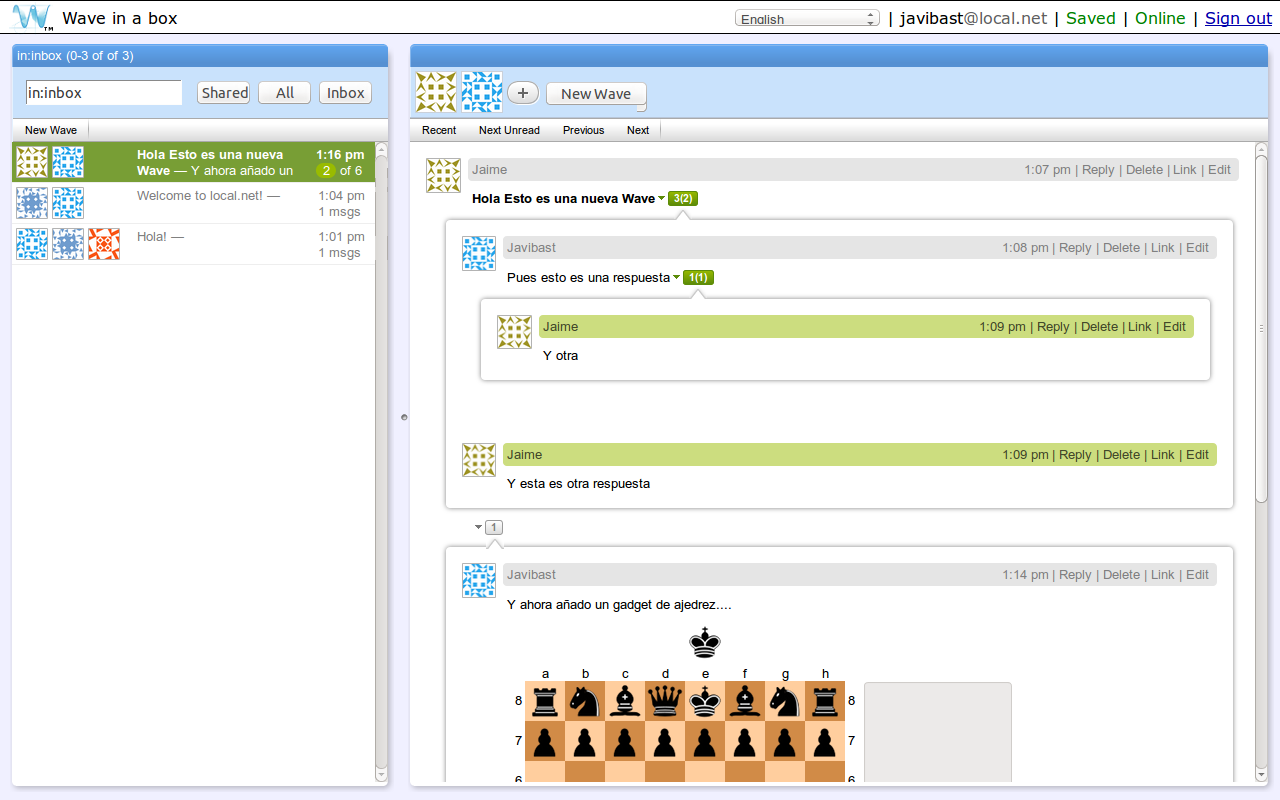
\includegraphics[keepaspectratio, scale=0.3]{Media/Captures/WIAB_Server.png}
      \caption{Cliente Wave In A Box}
      \label{fig:wiab_client}
    \end{figure} 

\section{Edición Colaborativa en Tiempo Real}

En esta sección veremos algunas de las soluciones disponibles actualmente que, al igual que Wave, permiten editar contenido de forma colaborativa y en tiempo real. Sin embargo, todas estas plataformas utilizan una arquitectura de servidor centralizado para ofrecer estas funcionalidades, mientras que Wave utiliza una arquitectura federada en la que no existe un servidor central (Ver Sección \ref{sssec:federation}).

De esta manera, primero veremos las principales herramientas de desarrollo (APIs) más utilizadas actualmente, para después pasar a ver algunas de las plataformas que hacen uso de esta tecnología. En su mayoría son para web, aunque existen unas pocas para Android. 
	
	\subsection{APIs Centralizadas}
	
	La mayor parte del desarrollo de tecnologías de Colaboración en Tiempo Real (RTC) se realiza mediante APIs que son propiedad de determinadas compañias y que no utilizan una arquitectura federada, sino que toda la información pasa por un servidor central que controla el RTC. A continuación veremos algunas de las más utilizadas hoy en día.
	
	\subsubsection{Google Realtime API}\label{sssec:googleAPI}
	
	Google Realtime API \cite{ref:google_api} permite construir aplicaciones de colaboración en tiempo real utilizando la tecnología de Transformaciones Operacionales (OT) presente en Google Docs. Utiliza JavaScript para poder construir construir en nuestro cliente web un modelo de datos (Realtime Data Model) que se guarda en sus servidores y gestiona automaticamente los cambios realizados por cualquiera de los usuarios que colaboran en tiempo real. Estos cambios en el modelo son notificados al servidor y al resto de usuarios mediante eventos que se lanzan al modificar los datos sobre los que se está colaborando. Para utilizarlo es necesario tener cuenta en la Consola de Desarrolladores de Google y activar el uso de esta API con nuestras credenciales de usuario.
	
	\subsubsection{Microsoft RTC Client API}
	
	Microsoft RTC Client API	 \cite{ref:microsoft_api} permite construir aplicaciones que permitan realizar llamadas de audio/video o sesiones de mensajería instantánea (IM) de texto por Internet y en tiempo real. Las aplicaciones se deben escribir en C++ o Visual Basic y pueden ser utilizadas tanto en PC como en dispositivos móviles siempre que ejecuten un sistema operativo Windows.
	
	\subsubsection{WebRTC}
	
	WebRTC \cite{ref:webRTC} (Web Real-Time Communication) es un API open-source (bajo licencia BSD) actualmente en desarrollo por Google y la World Wide Web Consortium (W3C) y que pretende dotar a los navegadores web de capacidades de comnicación en tiempo real entre sí sin necesidad de plugins externos. En la actualidad se encuentra en su versión 1.0 y soporta los navegadores Firefox y Chrome. 
	
	
	\subsubsection{Mozilla TogetherJS}

	Mozilla TogetherJS \cite{ref:togetherjs_api} es una librería gratuita y de código libre (bajo licencia pública Mozilla v2) que permite añadir capacidades de colaboración en tiempo real a una página web. Utiliza WebRTC y webSockets para establecer comunicaciones peer-to-peer (P2P) entre dos o más navegadores Web. No proporciona alamcenamiento persistente de los datos y es necesario tener un Servidor que establezca la conexión. Con esta herramienta se puede editar texto en tiempo real (usando Transformaciones Operacionales), establecer chats de audio/video y sincronizar el contenido de los navegadores. Dispone de GitHub para contribuir a su desarrollo. 	
	
	\subsubsection{ShareJS}

	ShareJS \cite{ref:shareJS} es una plataforma open-source (bajo licencia MIT) que dispone de un pequeño servidor basado en Node.js y una librería de cliente JavaScript que permiten la edición colaborativa de contenido mediante Transformaciones Operacionales. Permite actuar sobre objetos JSON o sobre texto plano. Dispone de GitHub para scontribuir a su desarrollo.
	
	\subsubsection{Goodow}
	
	Goodow \cite{ref:goodow} es un framework open-source de reciente desarrollo que proporciona un API muy similar a la de Google (Ver Sección \ref{sssec:googleAPI}) para colaboración en tiempo real mediante el uso de Transformaciones Operacionales. Dispone asimismo de dos clientes básicos para Android e iOS, utilizando una implementación del Servidor propia.	
	
	\subsection{Plataformas Web y Android}

	En las siguientes secciones veremos algunas de las plataformas Web y Android que hacen uso de tecnologías de Colaboración en Tiempo Real.	
	
	\subsubsection{Google Docs}
	
	Google Docs \cite{ref:google_docs} es la plataforma de Google para edición de documentos de forma colaborativa y en Tiempo Real usando su API Realtime (Ver Sección \ref{sssec:googleAPI}). Permite que varios usuarios con cuenta de Google creen y editen colaborativamente un documento a la vez. Puedes ver los cursores de cada usuario e interactuar con ellos mediante un chat. También permite escribir sugerencias a modo de notas en el margen sobre lo ya escrito. Dispone de versión web y móvil, pudiendo interactuar entre ellas sin problemas.
	
	\begin{figure}[H]
        \centering
        \begin{subfigure}[b]{0.6\textwidth}
                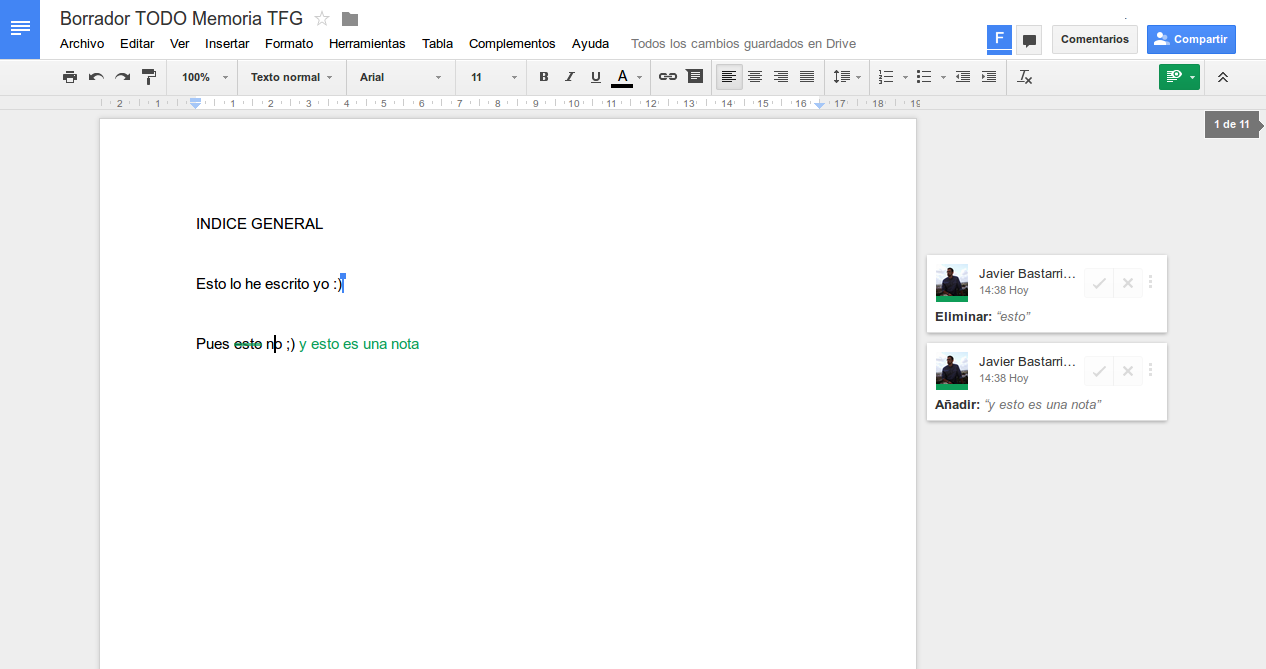
\includegraphics[width=\textwidth, height=6cm]{Media/Captures/googleDocsWeb.png}
                \caption{Interfaz Web}
                \label{fig:googleDocsWeb}
        \end{subfigure}
        ~
        \begin{subfigure}[b]{0.3\textwidth}
                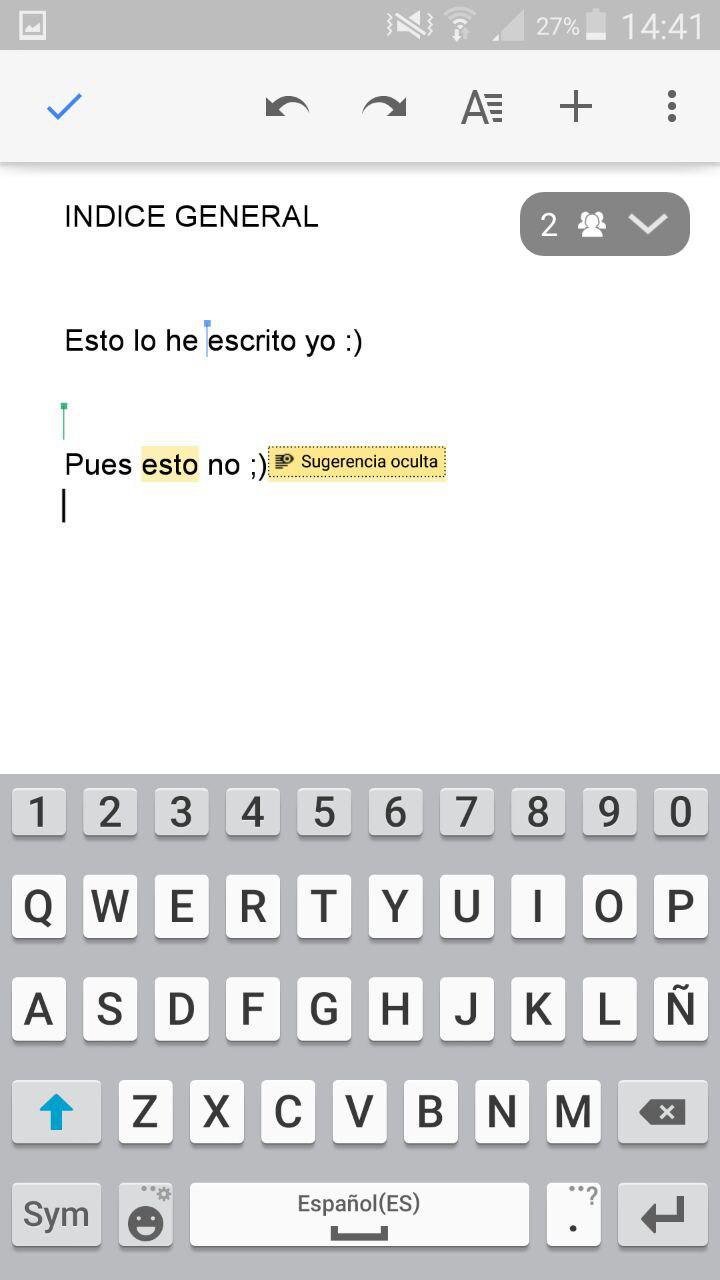
\includegraphics[width=\textwidth, height=7cm]{Media/Captures/googleDocsApp.jpg}
                \caption{Interfaz Android}
                \label{fig:googleDocsApp}
        \end{subfigure}
        \caption{Capturas de Google Docs}\label{fig:googleDocsCaptures}
	\end{figure}
	
	\subsubsection{Etherpad}
	
	Etherpad \cite{ref:etherpad} es un editor colaborativo en tiempo real open-source (bajo licencia Apache 2.0). Permite a varios autores editar a la vez un mismo documento de texto, resaltando en distintos colores lo editado por cada persona y con la opción de un chat para comunicarse entre sí. Existen múltiples servicios que hacen uso de este editor, siendo uno de las más conocidas TitanPad \cite{ref:titanpad}.
	
	\begin{figure}[H]
		\centering
			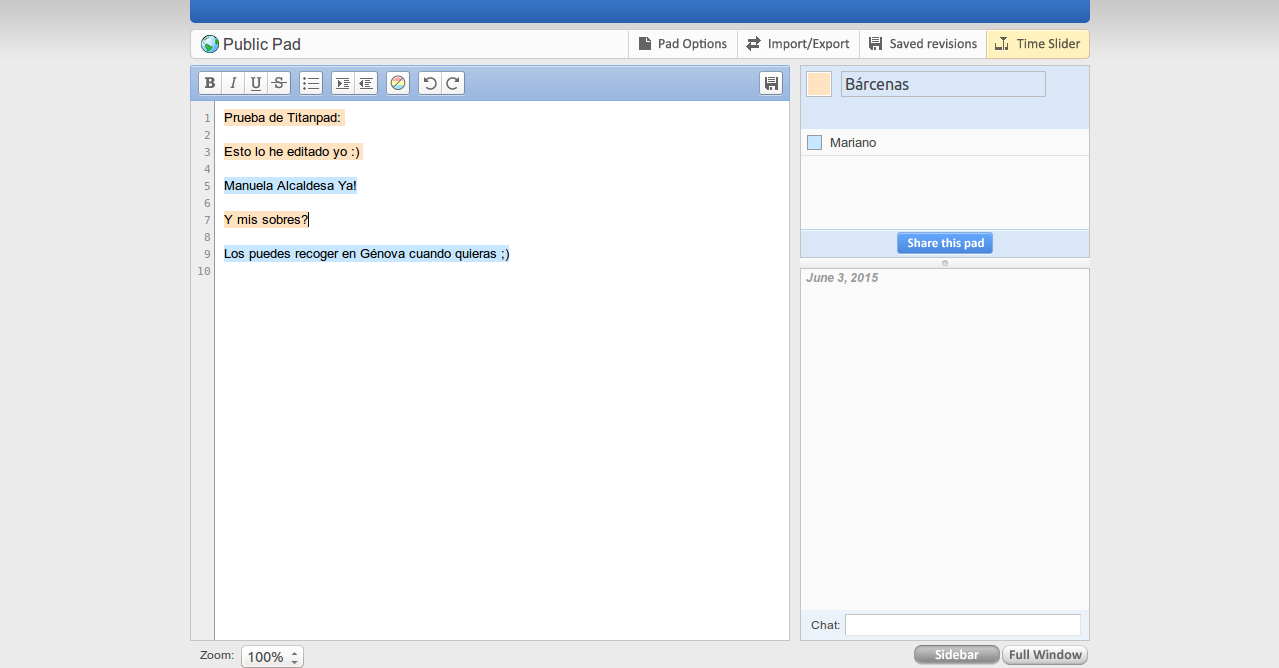
\includegraphics[keepaspectratio, scale=0.30]{Media/Captures/titanpadWeb.png}
		\caption{Captura de TitanPad: Ejemplo de uso de EtherPad}
		\label{fig:titanpad}
	\end{figure} 	
	
	\subsubsection{Colorillo}
	
	Colorillo \cite{ref:colorillo} es una aplicación web básica de dibujo colaborativo en tiempo real. Cualquier usuario puede empezar a dibujar sobre un nuevo lienzo en blanco con diversos colores y compartir este lienzo con otros usuarios para dibujar entre todos. De cada usuario podemos ver su procedencia aproximada sobre un mapa y el color que actualmente está utilizando. Existe también opción para chatear con otros usuarios. Los dibujos se pueden descargar y tienen todos licencia Creative Commons BY 3.0.
	
	\begin{figure}[H]
		\centering
			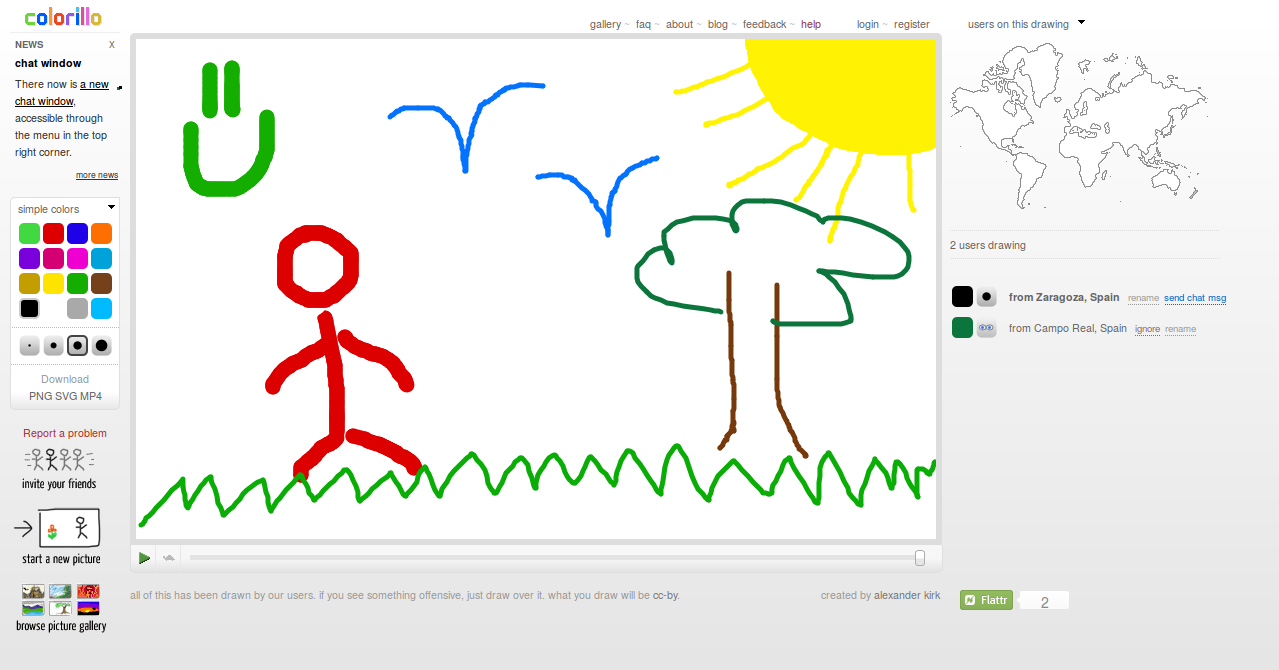
\includegraphics[keepaspectratio, scale=0.30]{Media/Captures/colorilloWeb.png}
		\caption{Captura de Colorillo}
		\label{fig:colorillo}
	\end{figure}  	
	
	\subsubsection{ShareLaTeX}
	
	ShareLaTeX \cite{ref:shareLatex} es un editor web colaborativo de documentos escritos en LaTeX en tiempo real. Permite elaborar documentos LaTeX esntre varias personas, ofreciendo una interfaz que incluye una previsualización del resultado en PDF. Desde 2014 es open-source (bajo licencia AGPL v3) y cualquiera puede descargarselo de GitHub e instalar su propio servidor (escrito en Node.js) de ShareLaTeX. En su web ofrecen también opciones de pago con extras como un control de versiones o sincronización con Dropbox.
	
	\begin{figure}[H]
		\centering
			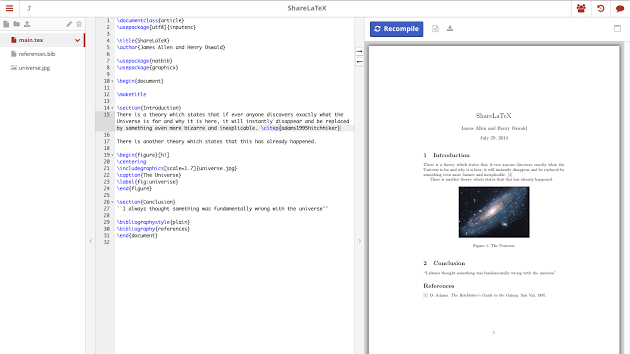
\includegraphics[keepaspectratio, scale=0.60]{Media/Captures/shareLatexWeb.png}
		\caption{Captura de ShareLaTeX}
		\label{fig:shareLaTeX}
	\end{figure}  
		
	\subsubsection{Samepage}
	
	Samepage \cite{ref:samepage} es una aplicación, tanto para web como para plataformas móviles (Android e iOS), que permite crear páginas que pueden ser editadas de forma colaborativa y en tiempo real por múltiples usuarios. Para ello es necesario solo es tener una cuenta de samepage. Tanto el cliente web como el móvil permiten interactuar entre ellos para crear nuevas páginas, editar texto y hacer comentarios, aunque la versión web permite también añadir tablas, imágenes y archivos.
	
	\begin{figure}[H]
        \centering
        \begin{subfigure}[b]{0.6\textwidth}
                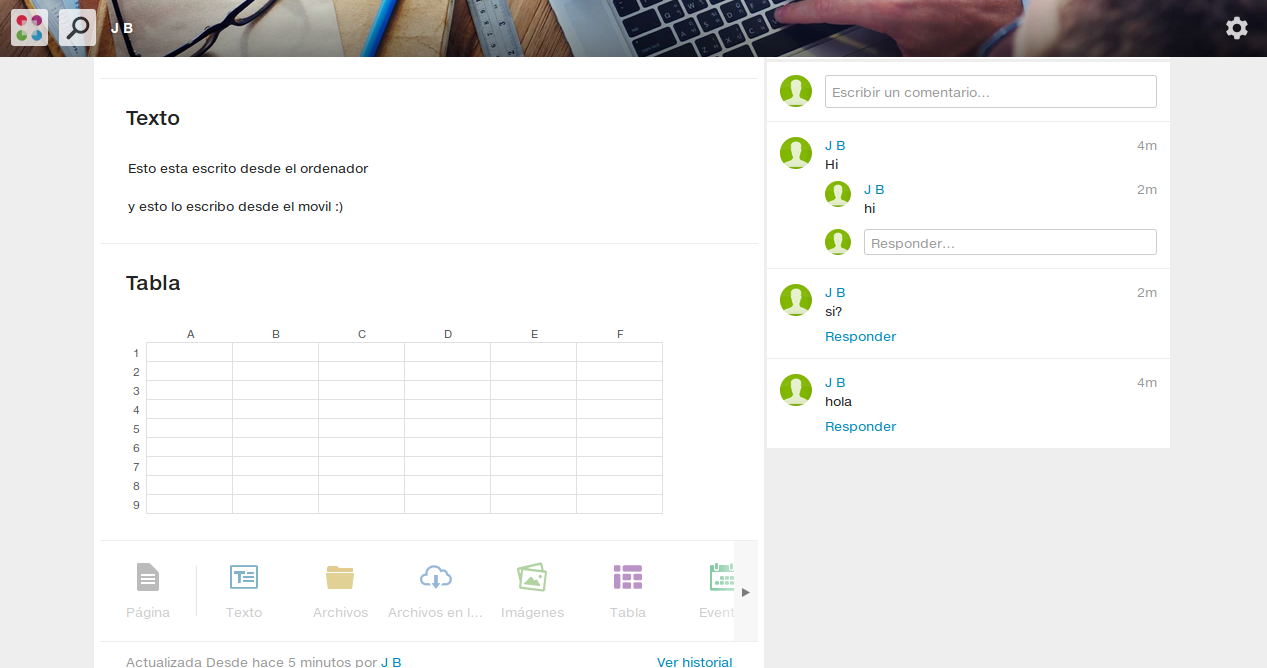
\includegraphics[width=\textwidth, height=6cm]{Media/Captures/samepageWeb.png}
                \caption{Interfaz Web}
                \label{fig:samepageWeb}
        \end{subfigure}
        ~
        \begin{subfigure}[b]{0.3\textwidth}
                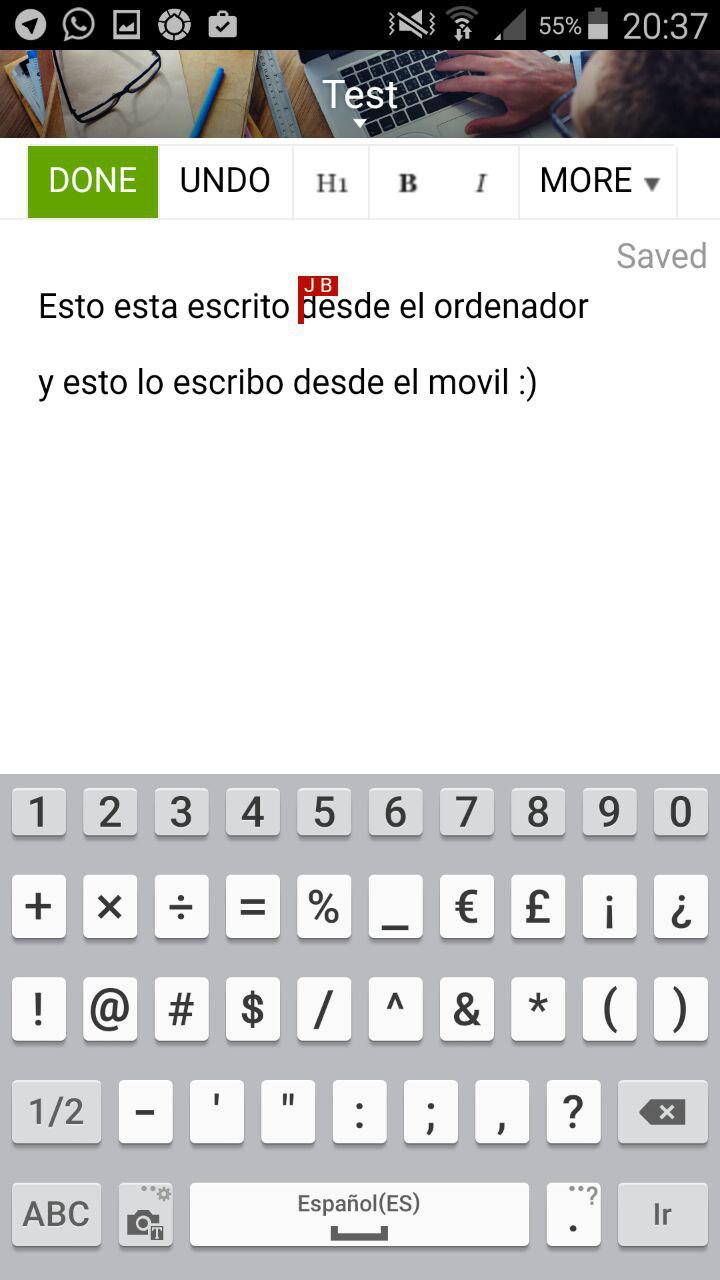
\includegraphics[width=\textwidth, height=7cm]{Media/Captures/samepageApp.jpg}
                \caption{Interfaz Android}
                \label{fig:samepageApp}
        \end{subfigure}
        \caption{Capturas de Samepage}\label{fig:samepageCaptures}
	\end{figure}
	
	
	\subsubsection{Quip}
	
	Quip \cite{ref:quip} es una aplicación para dispositivos móviles (Android e iOS) desarrollada con el objetivo de aumentar la productividad en los trabajos en grupo. Permite elaborar documentos, hojas de cálculo y listas de tareas compartidas y editables de forma colaborativa en tiempo real, pudiendo realizar tambien comentarios sobre ellas. Dispone también de una versión web, pero es necesario tener cuenta para usarla.
	
	\begin{figure}[H]
        \centering
        \begin{subfigure}[b]{0.3\textwidth}
                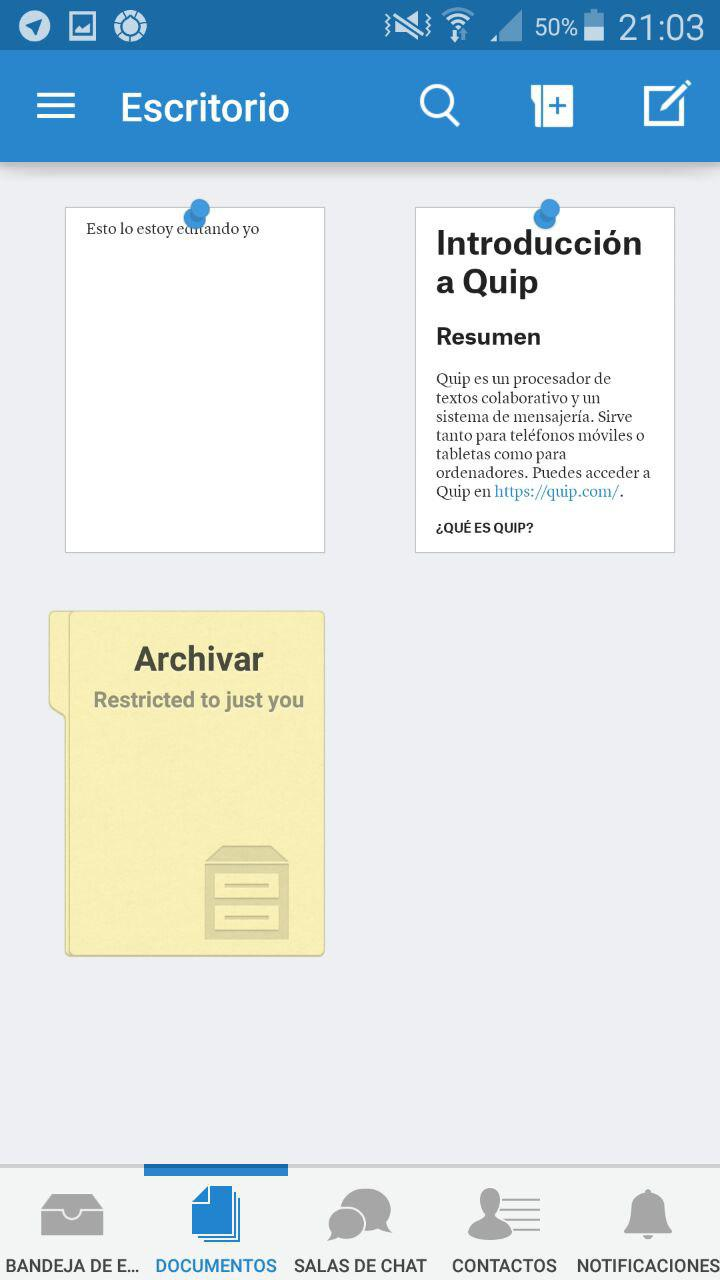
\includegraphics[width=\textwidth]{Media/Captures/quipDesktop.jpg}
                \caption{Escritorio}
                \label{fig:quipDesktop}
        \end{subfigure}
        ~
        \begin{subfigure}[b]{0.3\textwidth}
                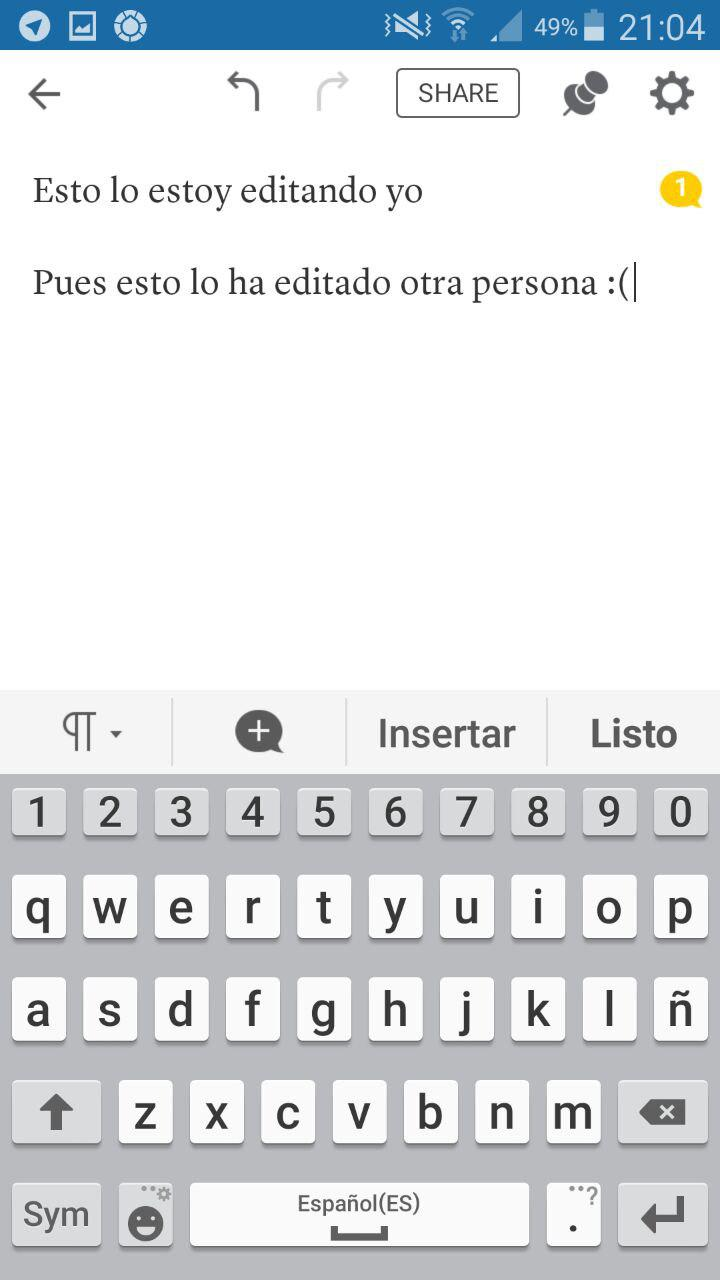
\includegraphics[width=\textwidth]{Media/Captures/quipEdit.jpg}
                \caption{Edición de texto}
                \label{fig:quipText}
        \end{subfigure}
        ~
        \begin{subfigure}[b]{0.3\textwidth}
                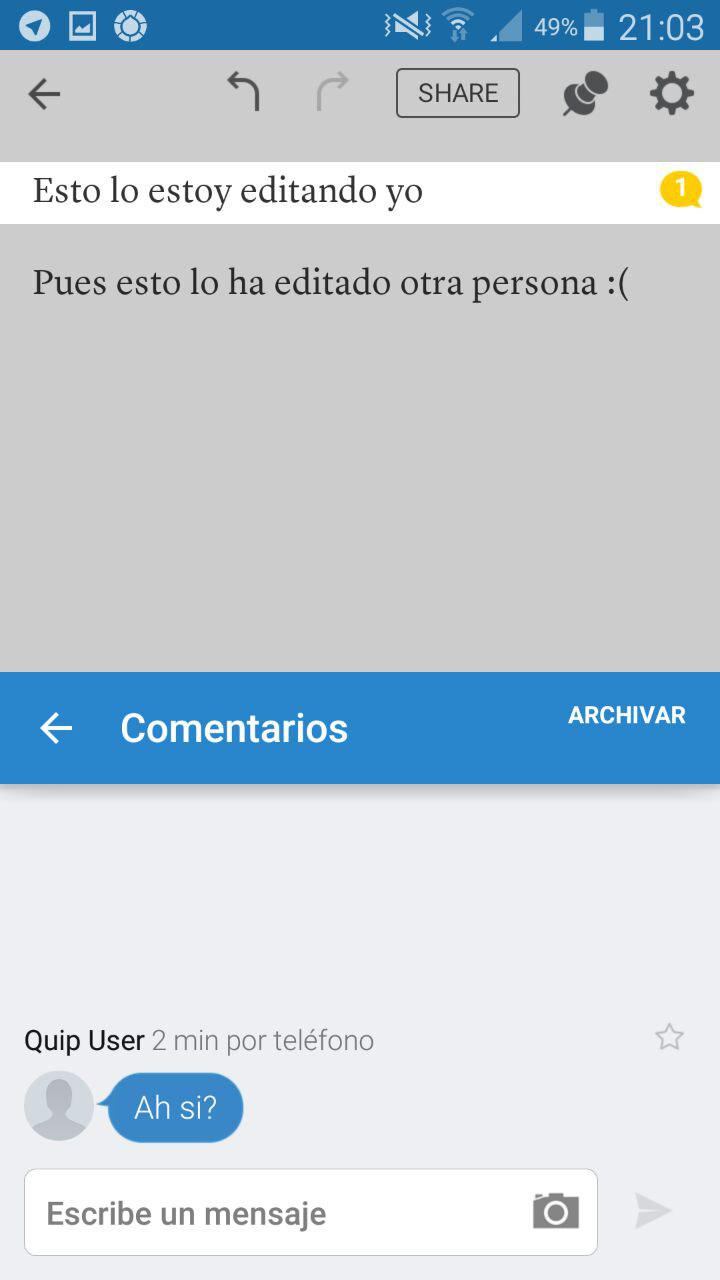
\includegraphics[width=\textwidth]{Media/Captures/quipComment.jpg}
                \caption{Comentarios}
                \label{fig:quipComments}
        \end{subfigure}
        \caption{Capturas de Quip}\label{fig:quipCaptures}
	\end{figure}
	
	

\section{Aplicación Android: DemoCritics}

En esta sección exploraremos algunas de las principales aplicaciones informáticas que existen en la actualidad destinadas a la participación ciudadana en propuestas, lectura de programas electorales o divulgación de candidaturas.

\subsection{Programas Políticos}

En la actualidad no existe ningún tipo de aplicación móvil orientada a debatir los programas electorales de los partidos políticos en su conjunto. Concretamente no existe ningún tipo de plataforma que agrupe en un solo sitio los programas electorales de las diferentes candidaturas.
Lo más parecido que hemos podido encontrar han sido aplicaciones elaboradas por un partido político, orientadas a dar a conocer su candidatura. En ellas podemos ver normalmente, entre otros, a presentación de candidatura, vídeos propagandísticos y el programa electoral. 

Pasamos ahora a analizar algunas de las aplicaciones móviles encontradas, identificando en cada caso aspectos e ideas que nos han resultado positivos y negativos.

\subsubsection{UPyD Parla}
La aplicación presenta al candidato de UpyD Carlos Alt Bustelo para la alcaldía de Parla. Se trata de una alicación divulgativa donde podemos conocer todo lo esencial de la candidatura de UpyD para las elecciones del municipio de Parla en Mayo de 2015: los candidatos, el programa, vídeos, etc.

\begin{figure}[H]
        \centering
        \begin{subfigure}[b]{0.3\textwidth}
                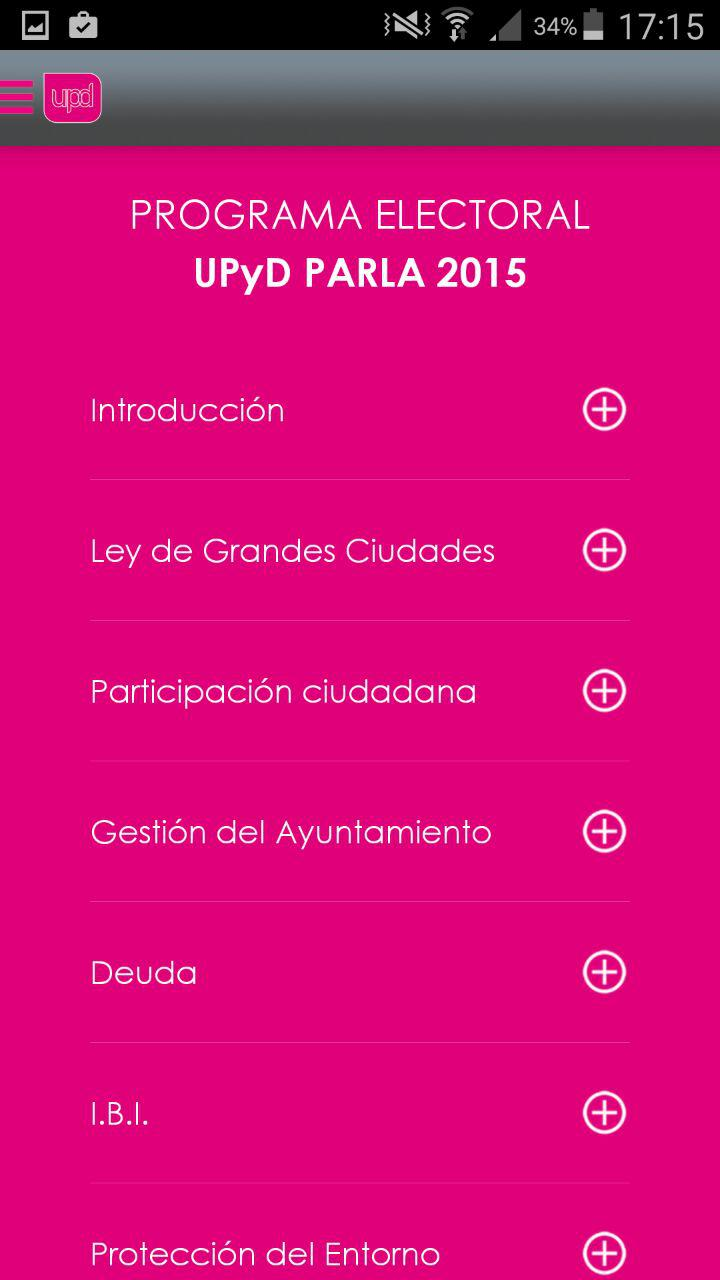
\includegraphics[width=\textwidth]{Media/Captures/UPyDParlaIndex.jpg}
                \caption{Indice Programa}
                \label{fig:upydIndex}
        \end{subfigure}
        ~
        \begin{subfigure}[b]{0.3\textwidth}
                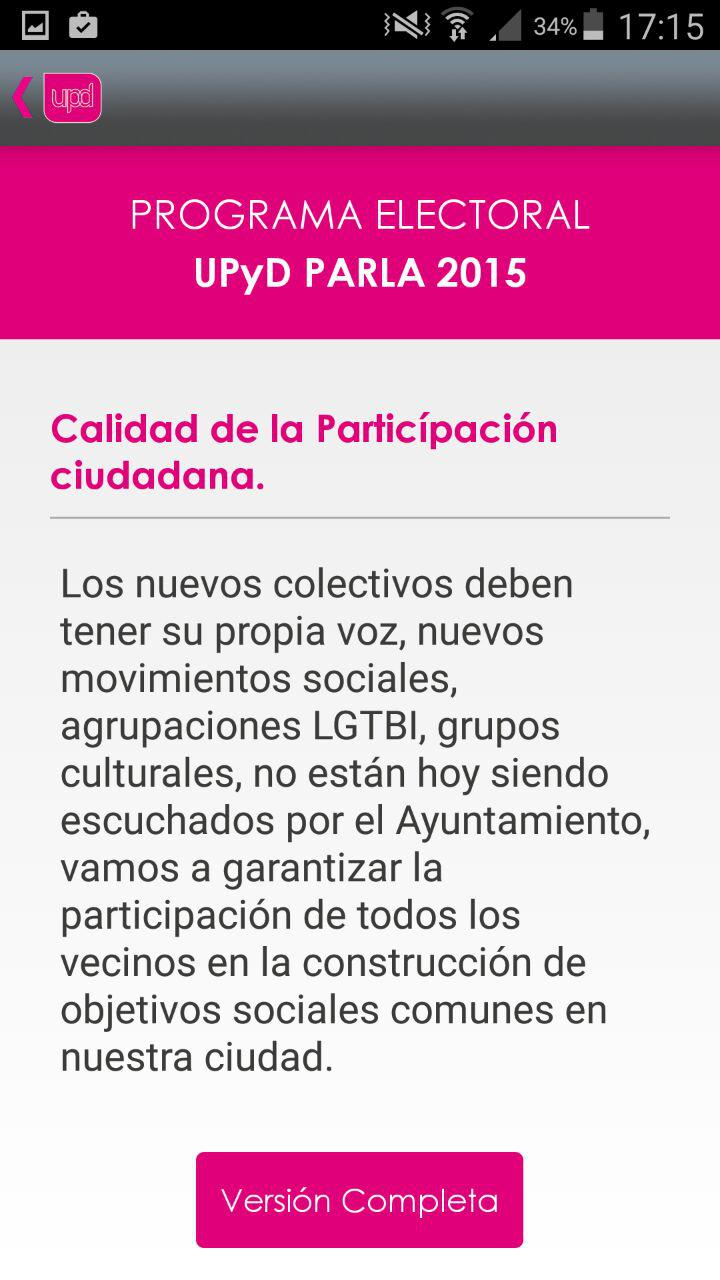
\includegraphics[width=\textwidth]{Media/Captures/UPyDParlaSection.jpg}
                \caption{Sección Programa}
                \label{fig:upydSection}
        \end{subfigure}
        ~
        \begin{subfigure}[b]{0.3\textwidth}
                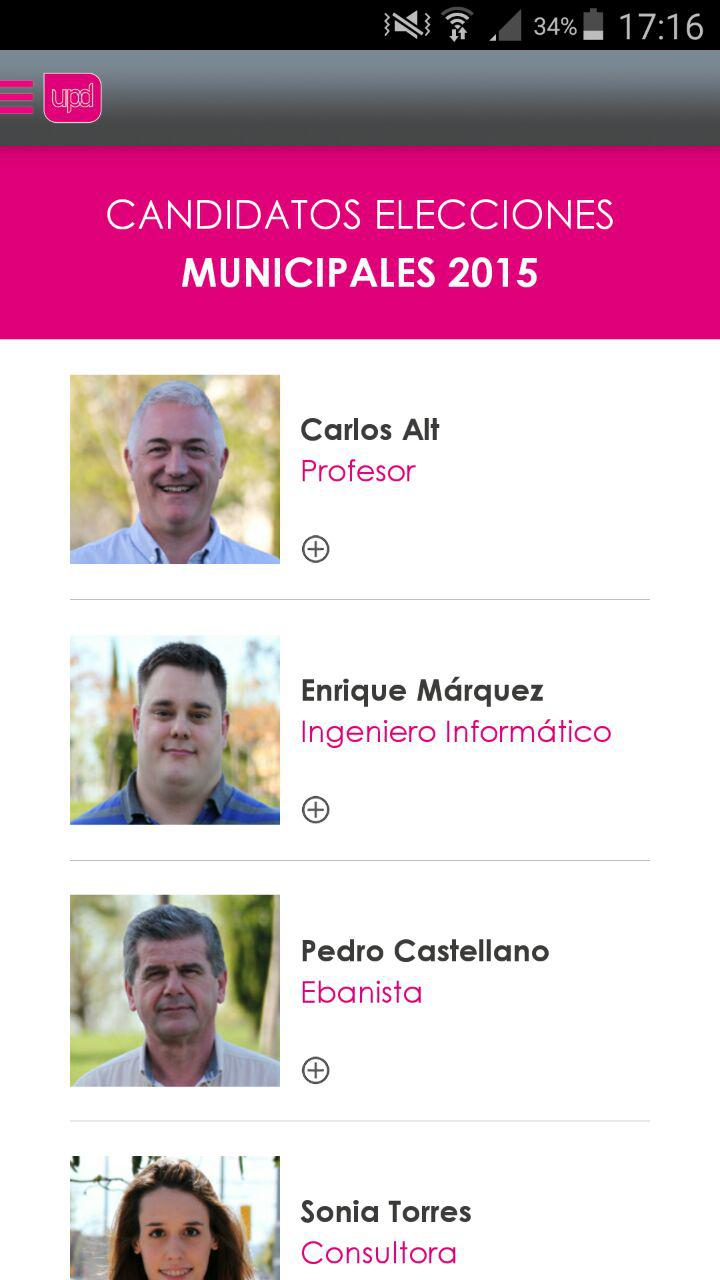
\includegraphics[width=\textwidth]{Media/Captures/UPyDParlaCandidates.jpg}
                \caption{Candidatos}
                \label{fig:upydCandidates}
        \end{subfigure}
        \caption{Capturas de UPyD Parla}\label{fig:upydCaptures}
\end{figure}

 - \underline{Aspectos positivos}:

\begin{itemize}
	\item 
	\item Presentación de Programa Electoral estructurado con Indice inicial.
	\item El Programa se lee dentro de la app, no nos lleva a leer el programa en PDF de la web. 
	\item Presentación de una Sección del Programa Electoral de forma resumida, teniendo la opción de leer la sección entera al pulsar un botón.
\end{itemize}

 - \underline{Aspectos negativos}:

\begin{itemize}
	\item Posee una sección llamada ''Memes'' cuyo nombre no se entiende ya que se limita a mostrar carteles propagandísticos de la candidatura. 
\end{itemize}

\subsubsection{$\sharp$RecuperaCórdoba}
Esta app presenta la candidatura de Pedro García de Izquierda Unida a la provincia de Córdoba, informando de su propuesta de gobierno de forma resumida. En la aplicación podremos encontrar la lista de los candidatos propuestos a la comunidad cordobesa, el programa electoral de la formación, las propuestas del partido, noticias de última hora y vídeos.

\begin{figure}[H]
        \centering
        \begin{subfigure}[b]{0.3\textwidth}
                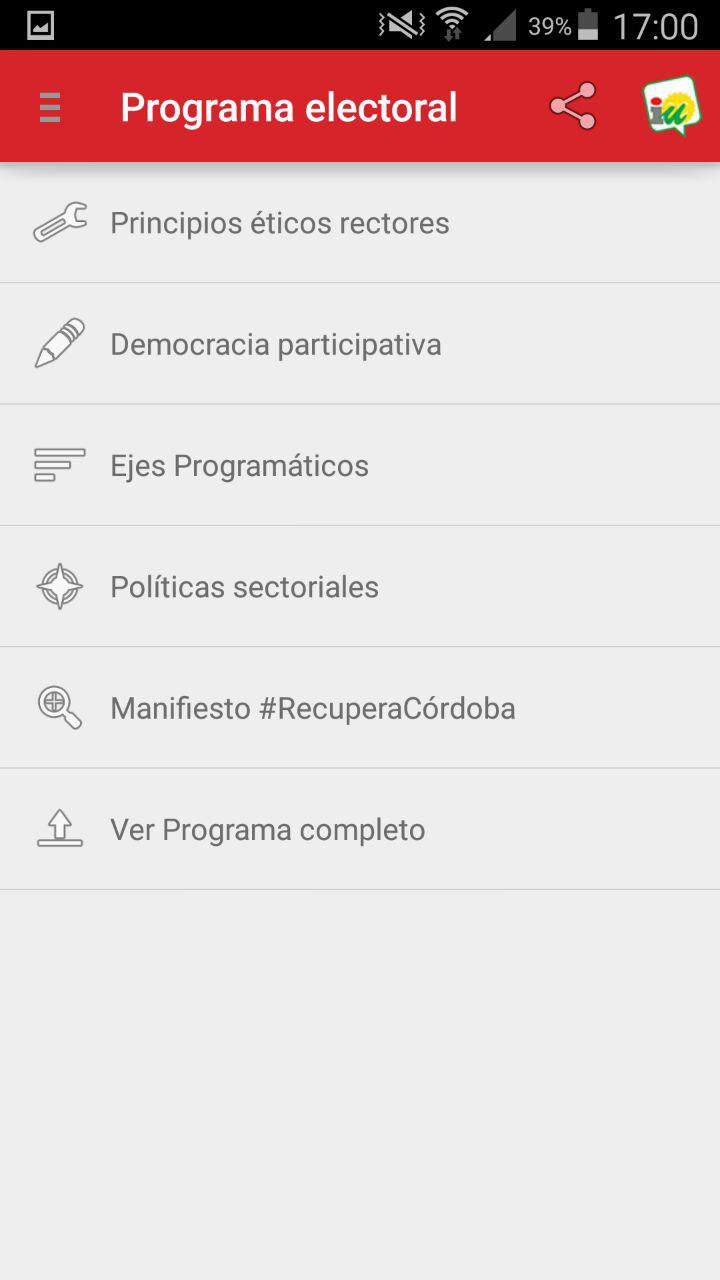
\includegraphics[width=\textwidth]{Media/Captures/IURecuperaCordoba.jpg}
                \caption{Indice Programa}
                \label{fig:iuIndex}
        \end{subfigure}
        ~
        \begin{subfigure}[b]{0.3\textwidth}
                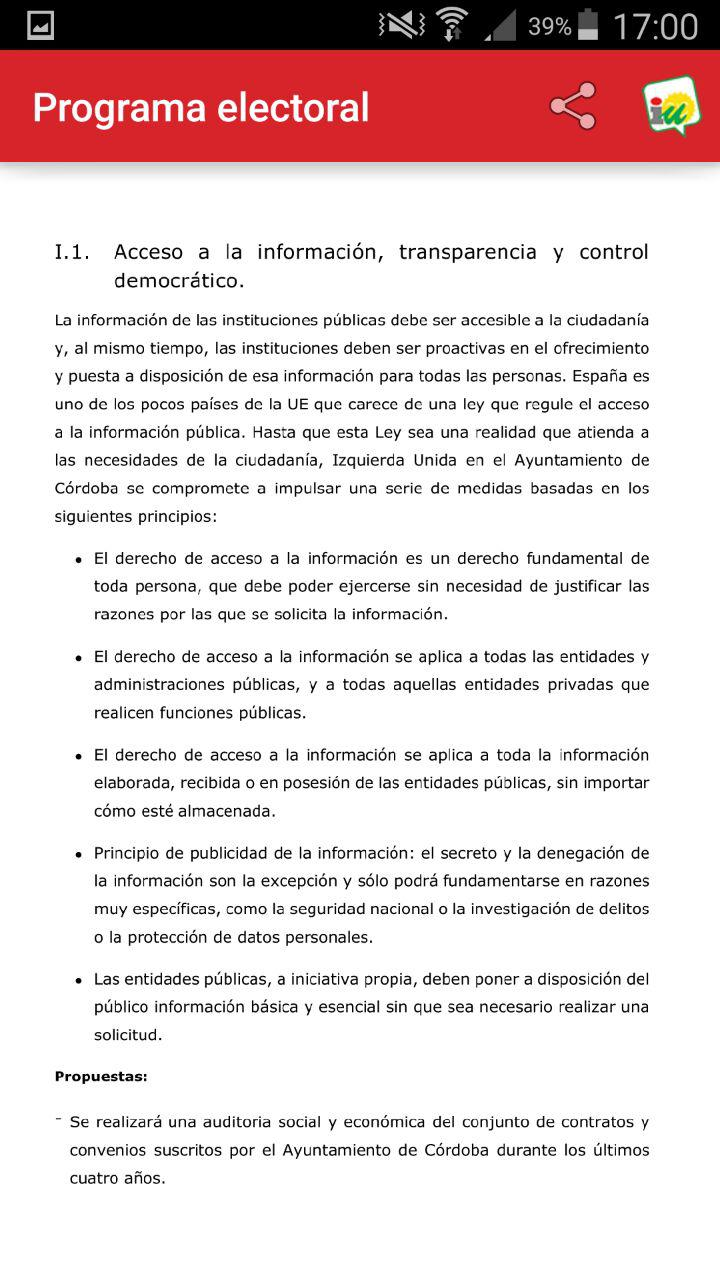
\includegraphics[width=\textwidth]{Media/Captures/IURecuperaCordobaSection.jpg}
                \caption{Sección Programa}
                \label{fig:iuSection}
        \end{subfigure}
        ~
        \begin{subfigure}[b]{0.3\textwidth}
                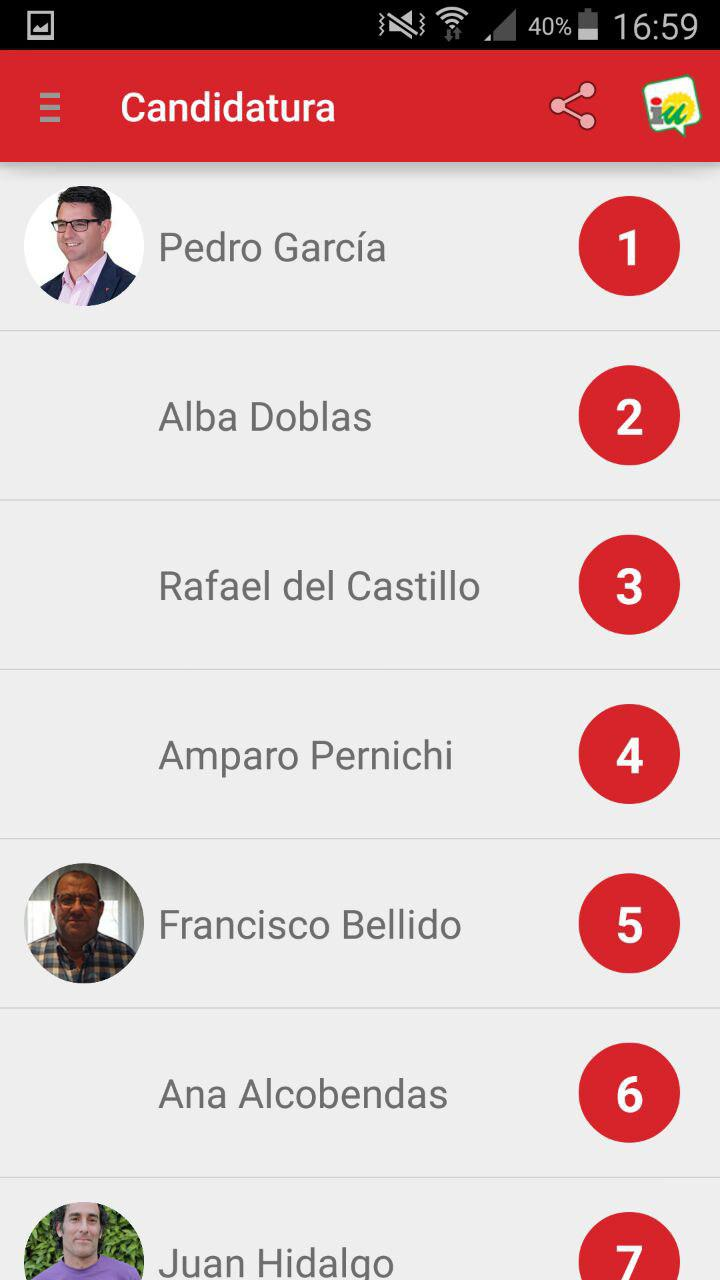
\includegraphics[width=\textwidth]{Media/Captures/IURecuperaCordobaCandidates.jpg}
                \caption{Candidatos}
                \label{fig:iuCandidates}
        \end{subfigure}
        \caption{Capturas de $\sharp$IURecuperaCórdoba}
        \label{fig:iuRecuperaCordoba}
\end{figure}

 - \underline{Aspectos positivos}:

\begin{itemize}
	\item Interfaz limpia y sencilla de diseño plano.
	\item Consistencia en la aplicación: la información se presenta siempre en formato de lista ofreciendo los minimos datos necesarios sin sobrecargar de información al usuario.
	\item Menú lateral disponible en cualquier pantalla con las principales acciones de la aplicación: Candidatos, Programa, Videos y Noticias.
	\item El programa electoral está estructurado en un indice primer nivel y a veces con segundo nivel.
	\item Aporta la opción de ver el programa completo. 
\end{itemize}

 - \underline{Aspectos negativos}:

\begin{itemize}
	\item Utiliza a veces iconos cuyo proposito no se entiende: ¿Un avión de papel para noticias? ¿Un ''a>z'' para la lista de candidatos?
	\item Las distintas secciones se abren dentro de la aplicación, pero da acceso a una navegación lateral por las páginas del PDF del programa en cuestión.
	\item Si haces zoom en una sección no permite pasar de página.
\end{itemize}

\subsubsection{PSOE Andalucía}

Esta app presenta la candidatura del PSOE a la junta de Andalucía para las elecciones del 22 de Marzo, promocionando básicamente su programa electoral y a la candidata Susana Díaz. Permite también estar al día de noticias y eventos relacionados con dicha candidatura.

La navegación por el programa, aunque estructurada en un primer nivel, se realiza directamente visualizando páginas que parecen extraidas del programa en PDF.

\begin{figure}[H]
        \centering
        \begin{subfigure}[b]{0.3\textwidth}
                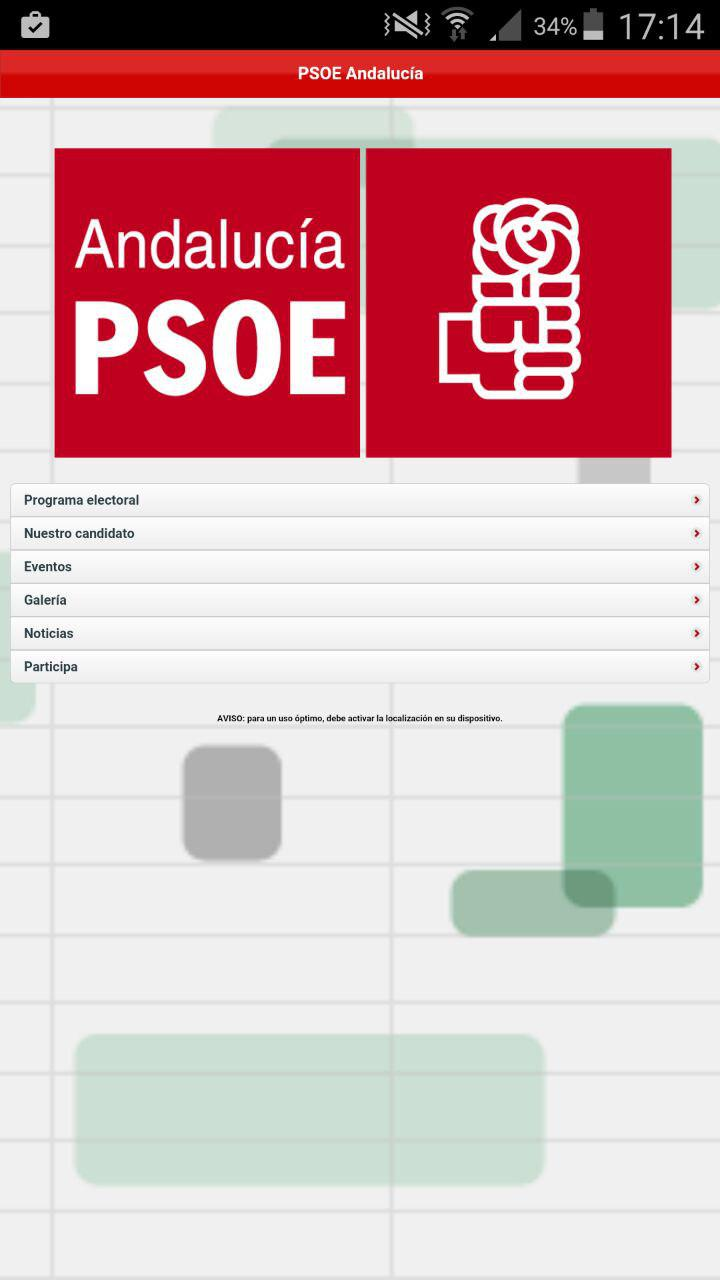
\includegraphics[width=\textwidth]{Media/Captures/psoeAndalucia.jpg}
                \caption{Pantalla Principal}
                \label{fig:psoePpal}
        \end{subfigure}
        ~
        \begin{subfigure}[b]{0.3\textwidth}
                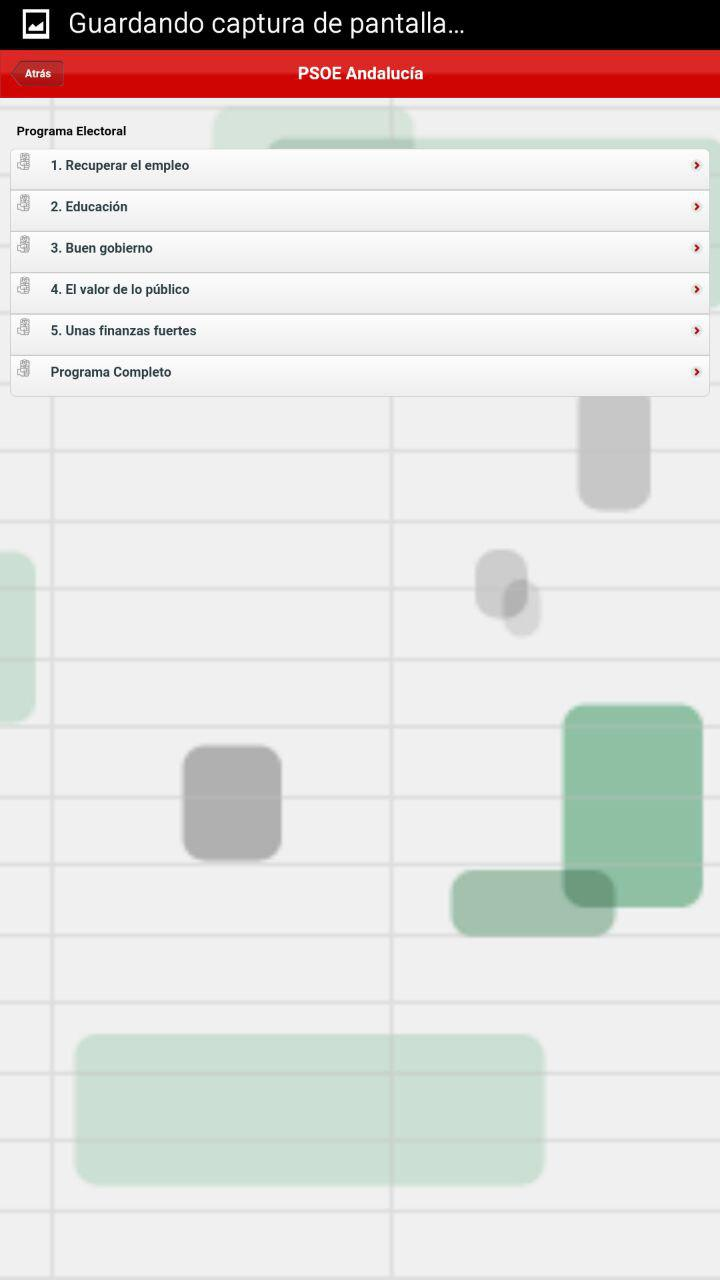
\includegraphics[width=\textwidth]{Media/Captures/psoeAndaluciaIndex.jpg}
                \caption{Indice Programa}
                \label{fig:psoeIndex}
        \end{subfigure}
        ~
        \begin{subfigure}[b]{0.3\textwidth}
                
\includegraphics[width=\textwidth]{Media/Captures/psoeAndaluciaSection.jpg}
                \caption{Sección Programa}
                \label{fig:psoeSection}
        \end{subfigure}
        \caption{Capturas de PSOE Andalucia}
        \label{fig:psoeAndalucia}
\end{figure}

 - \underline{Aspectos positivos}:

\begin{itemize}
	\item Posee un indice de primer nivel para estructurar el programa.
\end{itemize}

 - \underline{Aspectos negativos}:

\begin{itemize}
	\item La interfaz y los botones no se adaptan al tamaño de pantalla y permanecen de un tamaño pequeño que dificulta la interacción.
	\item El programa electoral se visiona en forma de una página que parece descargada directamente de la version PDF y que permanece en un tamaño pequeño e ilegible, no permitendo tampoco hacer zoom.
	\ En general, la interfaz parece hecha para una web más que para un móvil. 
\end{itemize}

\subsubsection{PP Canarias}

La delegación del Partido Popular en Canarias presenta su aplicación móvil para promocionar a sus candidatos para las elecciones autonómicas y municipales de Mayo de 2015. La aplicación nos avisará de los eventos electorales, podremos consultar los candidatos, novedades, galería de imágenes y por supuesto ver el programa electoral.

\begin{figure}[H]
        \centering
        \begin{subfigure}[b]{0.3\textwidth}
                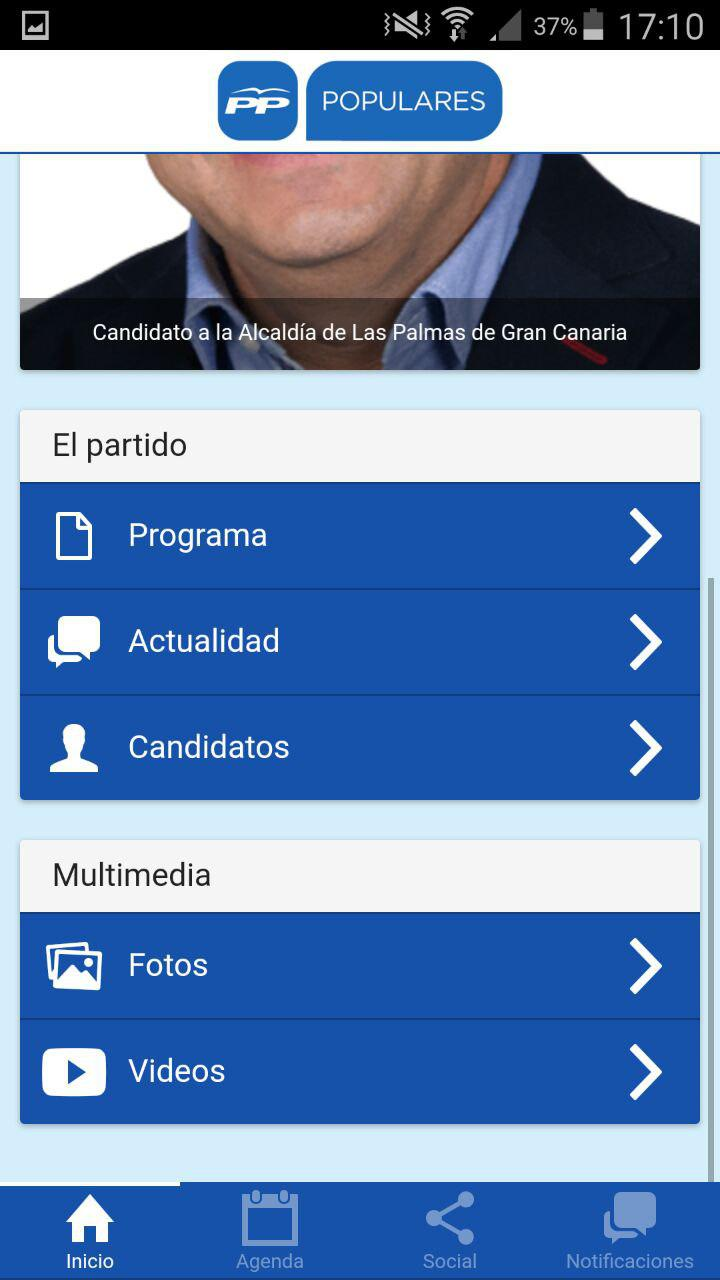
\includegraphics[width=\textwidth]{Media/Captures/ppCanarias.jpg}
                \caption{Pantalla Principal}
                \label{fig:ppIndex}
        \end{subfigure}
        ~
        \begin{subfigure}[b]{0.3\textwidth}
                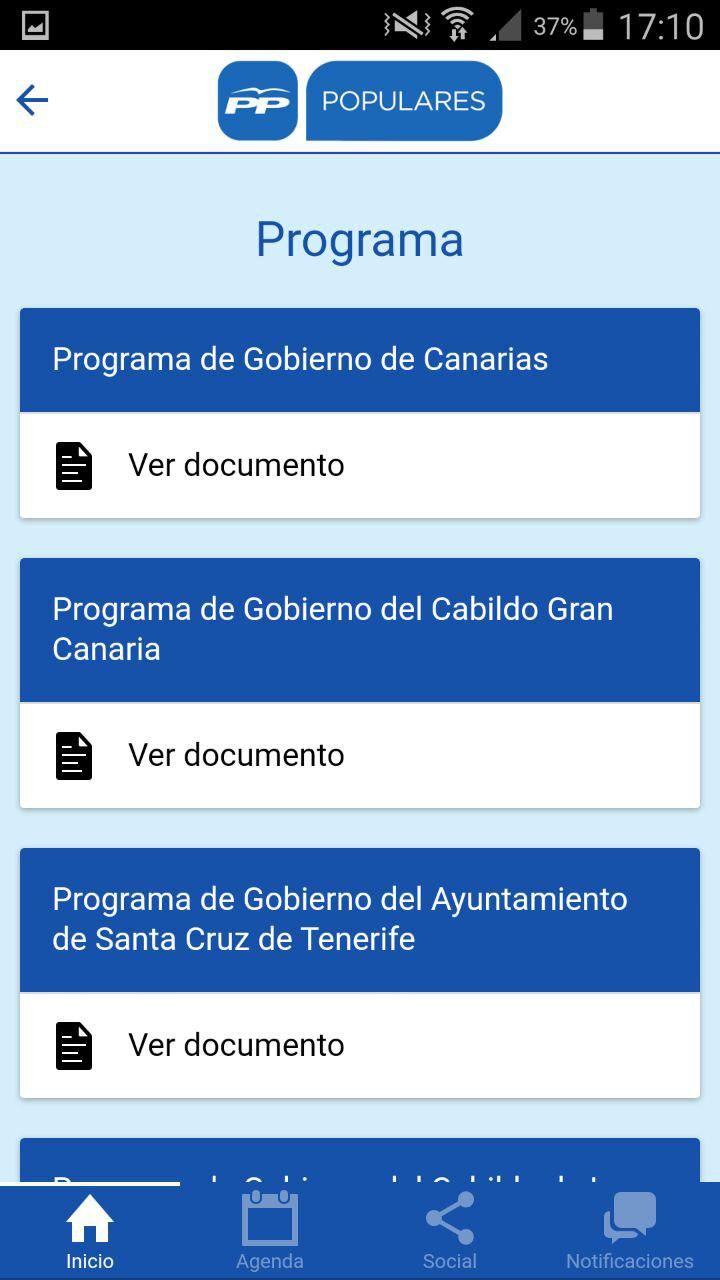
\includegraphics[width=\textwidth]{Media/Captures/ppCanariasProgram.jpg}
                \caption{Programas}
                \label{fig:ppPrograms}
        \end{subfigure}
        ~
        \begin{subfigure}[b]{0.3\textwidth}
                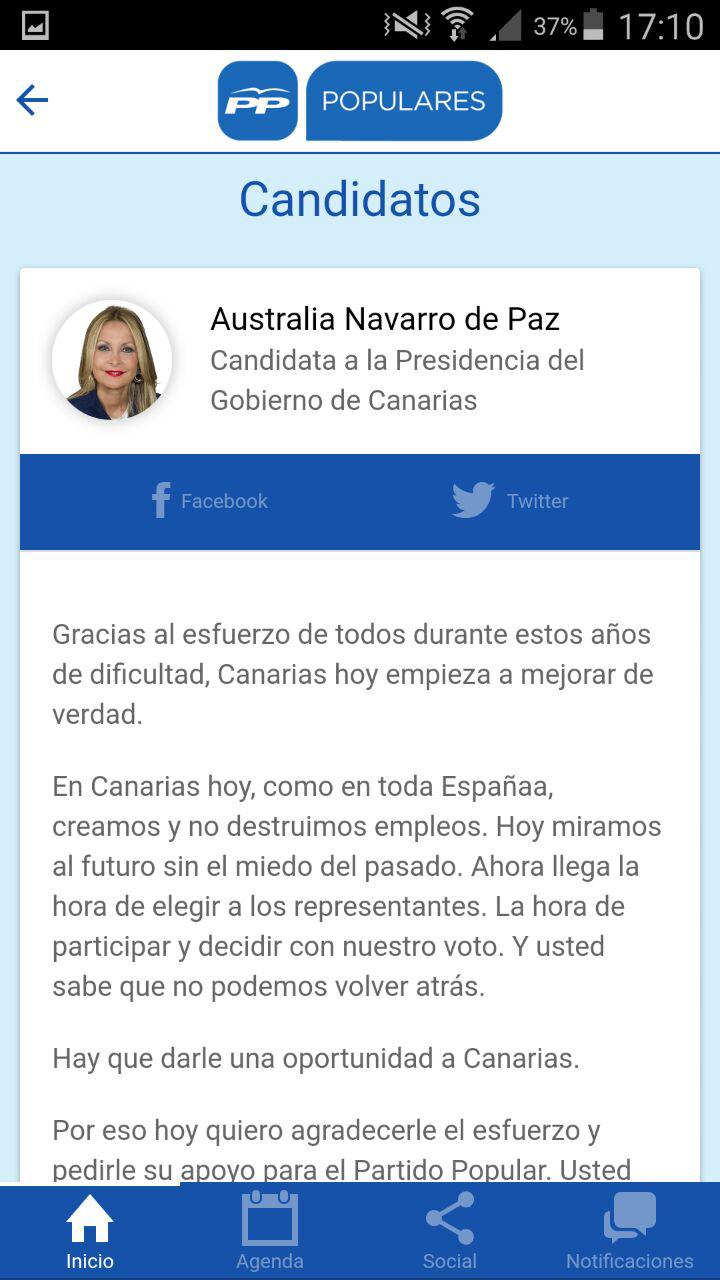
\includegraphics[width=\textwidth]{Media/Captures/ppCanariasCandidates.jpg}
                \caption{Candidatos}
                \label{fig:ppCandidates}
        \end{subfigure}
        \caption{Capturas de PP Canarias}
        \label{fig:ppCanarias}
\end{figure}

 - \underline{Aspectos positivos}:

\begin{itemize}
	\item Interfaz limpia y atractiva con una organización clara en secciones que aparecen en una barra inferior al estilo de iOS.
\end{itemize}

 - \underline{Aspectos negativos}:

\begin{itemize}
	\item Aunque dispone de una sección para programas electorales, no dispone de ellos en local, si no que te obliga a abrir un navegador para ver la versión entera en PDF.
	\item El problema de la barra inferior de menús es que quita espacio al contenido principal. Se podría haber puesto el menú en alun sitio menos intrusivo.
\end{itemize}

\subsection{Participación Ciudadana} \label{ssec:artProposals}

Centrándonos en la participación ciudadana ya sea mediante la generación de Propuestas, el desarrollo colaborativo de programas o la recogida de firmas, existen numerosos portales en internet y aplicaciones móviles destinadas a ello. Realizaremos un breve repaso a las aplicaciones más destacadas.

\subsubsection{Reddit}

Reddit \cite{ref:reddit} es una plataforma web de código libre donde los usuarios pueden crear temas, propuestas o compartir enlaces web a otros sitios. A primera vista puede parecer un foro, aunque la principal diferencia respecto a éste último radica en que otros usuarios pueden votar a favor o en contra de los enlaces, haciendo que el sistema los haga aparecer como más o menos destacados. De esta forma los temas de conversación, enlaces, o propuestas aparecerán en el orden que haya escogido la comunidad según la puntuación positiva o negativa que le hayan dado.
En principio el uso de reddit está destinado a todo tipo de temas, entre los que podemos encontrar algunos ejemplos fuertemente relacionados con la participación ciudadana. Es el caso de Plaza Podemos \cite{ref:plazaPodemos}: un espacio utilizado para que la ciudadanía pueda expresar sus propuestas, compartir noticias relacionadas con la actualidad política o debatir aquellos temas que más les preocupan. Así, aunque no seamos participantes de reddit, de un simple vistazo podemos saber qué es lo más debatido por la ciudadanía, las propuestas que quieren llevar a cabo en en el gobierno o cuáles son los temas que más les preocupan.

\begin{figure}[H]
\centering
\includegraphics[keepaspectratio, scale=0.30]{Media/Captures/plazaPodemos.png}
\caption{Plaza Podemos utilizando la plataforma Reddit}
\label{fig:plazaPodemos}
\end{figure}

 - \underline{Aspectos positivos}:

\begin{itemize}
	\item Opción de filtrado por tipos de contenido (propuestas, noticias...) y ordenación de distintas formas (nuevos, populares, activos...)
	\item Sistema de votación sencillo desde la propia previsualización del contenido mediante flechas (arriba y abajo), pudiendo ver entre ellas el número actual de votos.
\end{itemize}

 - \underline{Aspectos negativos}:

\begin{itemize}
	\item Para un usuario que lo usa por primera vez puede resultar confuso que haya contenido redactado con usuarios mezclado con enlaces a noticias externas.
\end{itemize}

\subsubsection{Change.org}

Change.org \cite{ref:changeOrg} es un portal web que permite lanzar múltiples peticiones de cambio en Internet. Podríamos definirlo como la evolución de la recogida de firmas en la calle: cualquiera puede realizar una petición para solicitar el apoyo de otros. Las personas que decidan apoyar la petición, dejarán sus datos personales y constarán entre el número de personas que han firmado a favor de la petición. Una vez que han alcanzado un número objetivo de apoyos se procede a entregar las firmas digitales al organismo, persona o entidad a la que va destinada la petición.

Por ejemplo: en mayo de 2011, en relación con las movilizaciones del Movimiento 15-M y Democracia Real Ya, y ante el desalojo por los Mossos de Esquadra se llevó a cabo la petición “Exige la dimisión fulminante del Conseller de Interior Felip Puig por la violencia utilizada en Pza. Catalunya”.

Desde su creación en 2007, Change.org ha logrado muchas de sus peticiones demandadas entre los que se incluyen la atención de pacientes con enfermedades complejas, protección sobre animales y medio ambiente, derechos públicos, leyes, etc.

\begin{figure}[H]
\centering
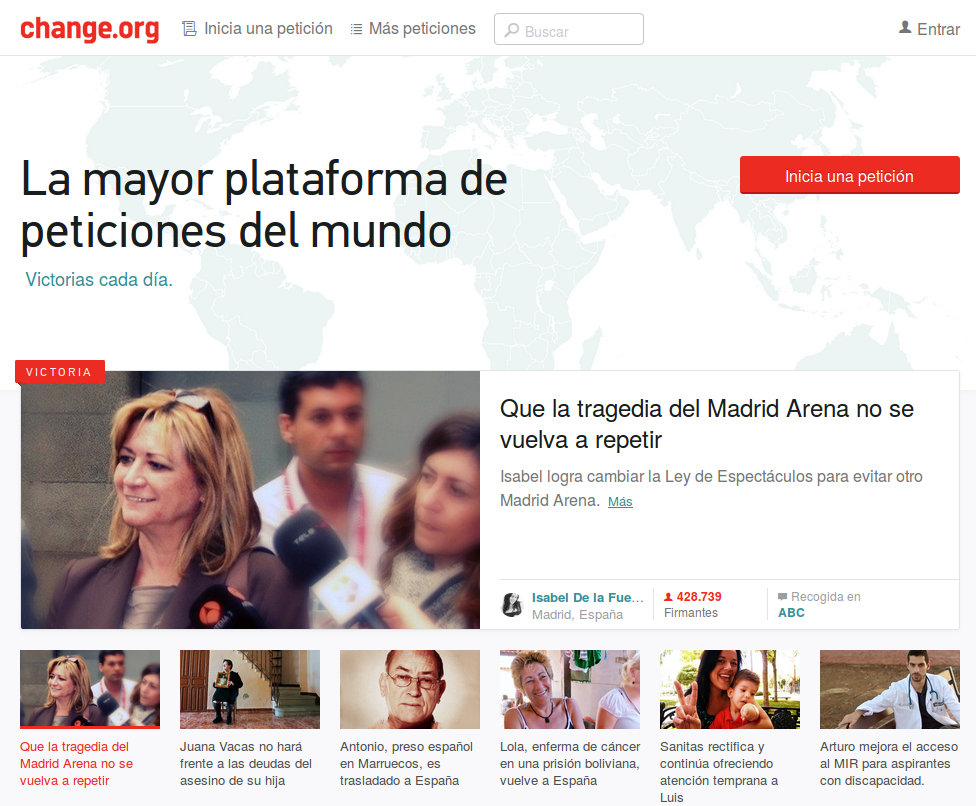
\includegraphics[keepaspectratio, scale=0.30]{Media/Captures/changeOrg.png}
\caption{Change.org · La mayor plataforma de peticiones del mundo}
\label{fig:changeOrg}
\end{figure}

 - \underline{Aspectos positivos}:

\begin{itemize}
	\item Página principal con peticiones cuyo objetivo de firmas se ha conseguido (''victoria'') y las más destacadas aun por conseguir.
	\item De cada petición se muestra un ''preview'' con los aspectos más destacados: foto, titulo, autor, número de firmas y fecha de creación.
\end{itemize}

 - \underline{Aspectos negativos}:

\begin{itemize}
	\item Aunque existen filtros para peticiones (Destacadas, Populares y Recientes) ¿de qué depende esta clasificación? No queda claro cómo se elige la opsición en dicha lista de peticiones,
\end{itemize}

\subsubsection{Programas Colaborativos de Ahora Madrid y Zaragoza en Común}

Para las pasadas elecciones municipales del 24 de Mayo, la candidatura de unidad popular Ahora Madrid, desarrolló una plataforma en la web para elaborar su programa electoral de forma colaborativa. En esta plataforma, cualquier usuario tenía la oportunidad de explorar las propuestas por categoría o por distrito. De tal forma que podría debatirlas, puntuarlas o crear sus propias propuestas. Así las propuestas más valoradas por la comunidad, serían llevadas al programa final para las elecciones municipales del 24 de Mayo.

El resultado final fue determinar las cinco propuestas más votadas que fueron incluidas en el programa final como medidas urgentes para realizar en los 100 primeros días de gobierno. 

\begin{figure}[H]
\centering
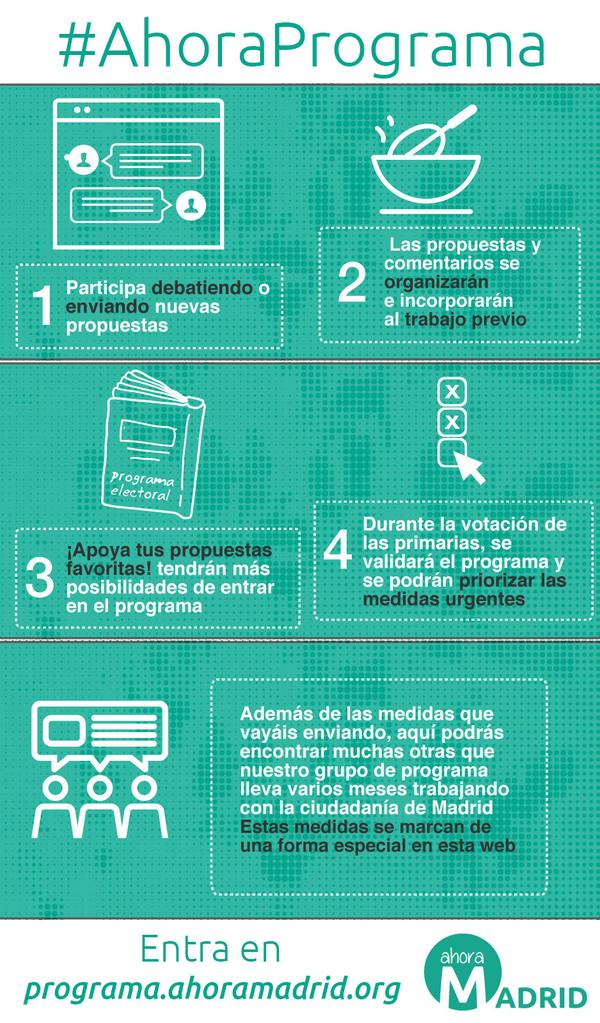
\includegraphics[keepaspectratio, scale=0.25]{Media/Captures/programaAhoraMadrid.jpg}
\caption{Creación colaborativa del programa de Ahora Madrid.}
\label{fig:programaAhoraMadrid}
\end{figure}

También utilizaron una plataforma similar en la candidatura zaragozana de unidad popular Zaragoza en Común \cite{ref:ganemosZaragoza}.

\begin{figure}[H]
\centering
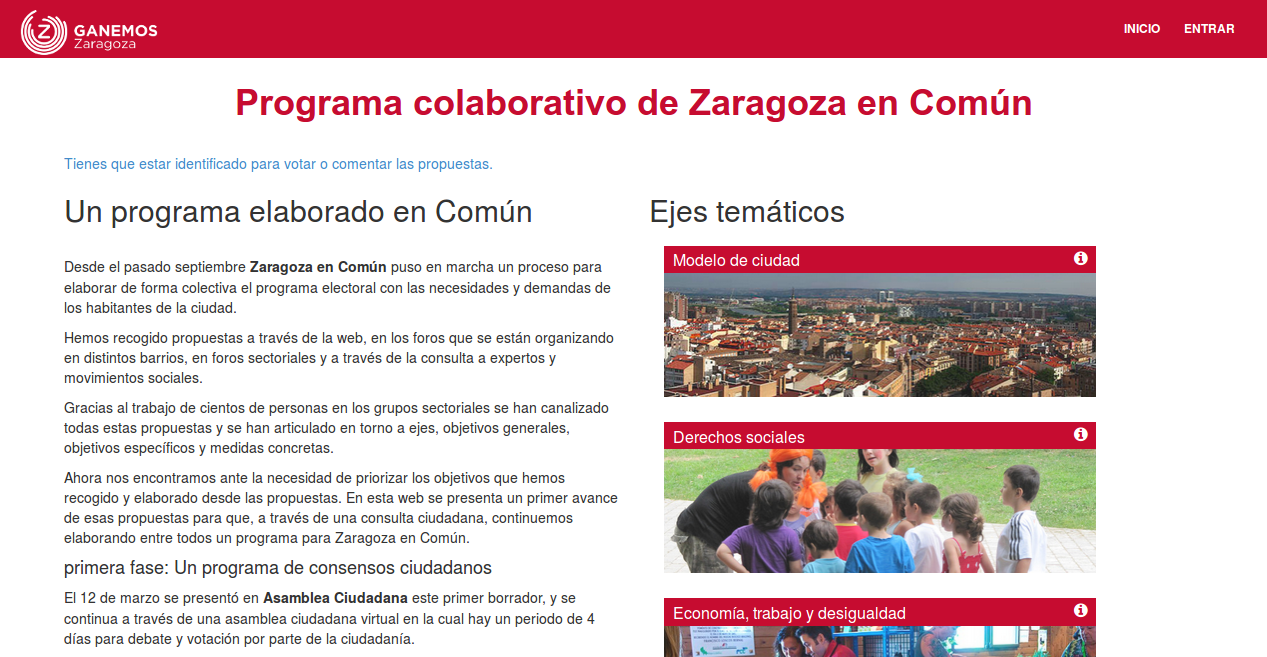
\includegraphics[keepaspectratio, scale=0.30]{Media/Captures/programaColaborativoGanemosZaragoza.png}
\caption{Creación colaborativa del programa de Zaragoza en Común.}
\label{fig:programaZaragozaEnComun}
\end{figure}

 - \underline{Aspectos positivos}:

\begin{itemize}
	\item Las propuestas están organizadas por distintos temas: ''Ejes temáticos'' en el caso de Zaragoza en Común y ''Areas y Objetivos'' en el caso de Ahora Madrid.
	\item En ambos casos se puede filtrar la lista de propuestas de distintas formas (''Más valoradas'', ''Más consenso'' y ''Más debatidas'') 
	\item En el ''preview'' de la propuesta se muestra el número de comentarios y el porcentaje de votos positivos en relación al número total de votos recibidos.
\end{itemize}

 - \underline{Aspectos negativos}:

\begin{itemize}
	\item En cada propuesta se muestra un número a la izquierda que no explica lo que significa (entendemos que es el número de votos a favor).
\end{itemize}

\subsubsection{Appgree}

Appgree\cite{ref:appgree} es una plataforma desarrollada con el objetivo de poner a grandes grupos de personas de acuerdo en poco tiempo. Está disponible tanto para web como para móviles y permite que sus usuarios lancen propuestas y debatan sobre cualquier tema pudiendo votar y alcanzar un consenso, obteniendo los resultados de dicha votación casi en tiempo real gracias a un algoritmo estadístico desarrollado por ellos llamado DemoRank\cite{ref:appgree_demoRank}.

En la aplicación podemos acceder a una lista de canales: que aglutinan encuestas, propuestas y preguntas (ya sea de respuesta abierta o de votación entre dos o mas opciones), pudiendo votar y ver los resultados actuales de votación y respuestas. Para fomentar la participación potencian mucho el uso tops de preguntas más candentes y recientes. Además se pueden compartir preguntas por redes sociales para aumentar su difusión.

\begin{figure}[H]
        \centering
        \begin{subfigure}[b]{0.3\textwidth}
                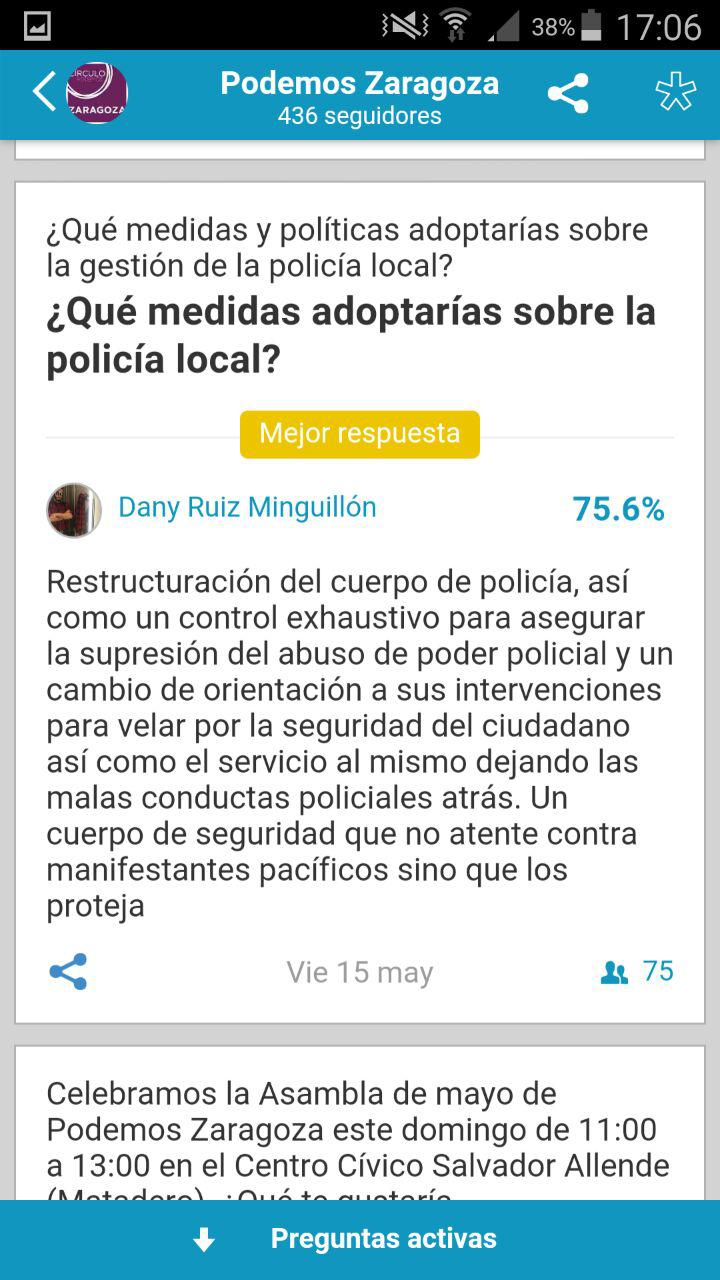
\includegraphics[width=\textwidth]{Media/Captures/appgreeChannel.jpg}
                \caption{Canal}
                \label{fig:appgreeChannel}
        \end{subfigure}
        ~
        \begin{subfigure}[b]{0.3\textwidth}
                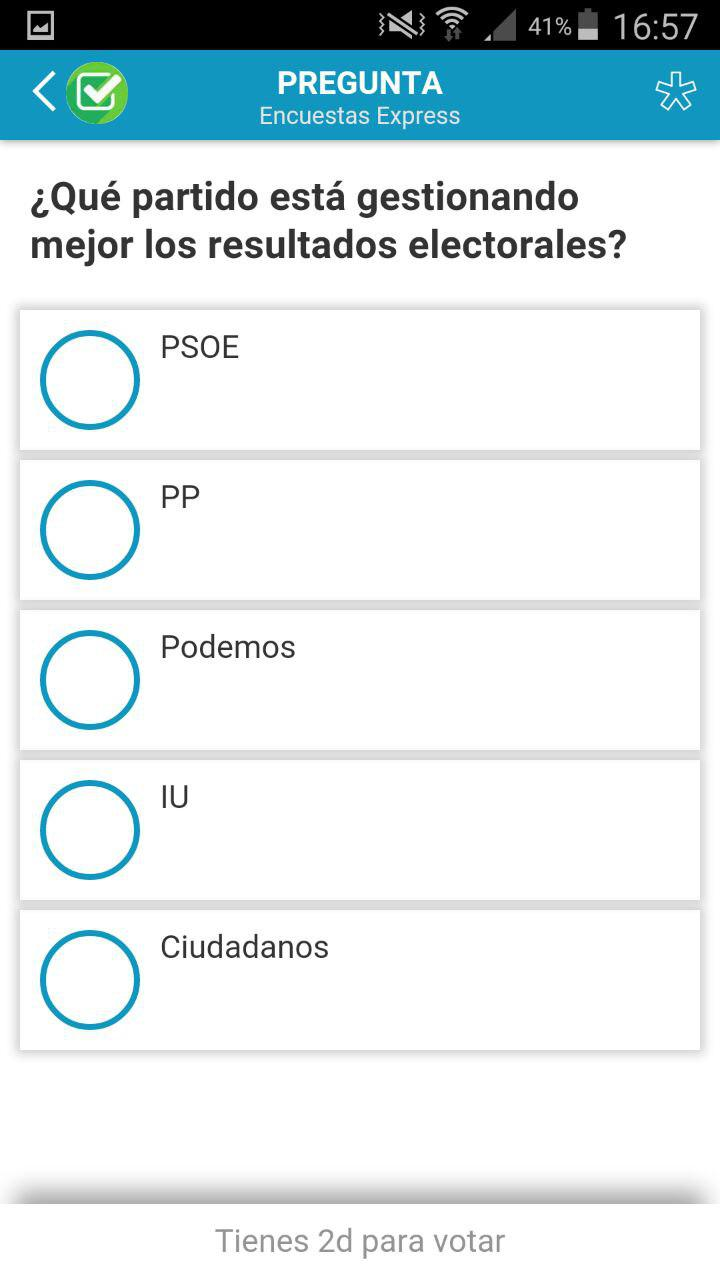
\includegraphics[width=\textwidth]{Media/Captures/appgreeQuestion.jpg}
                \caption{Pregunta Múltiple}
                \label{fig:appgreeQuestion}
        \end{subfigure}
        ~
        \begin{subfigure}[b]{0.3\textwidth}
                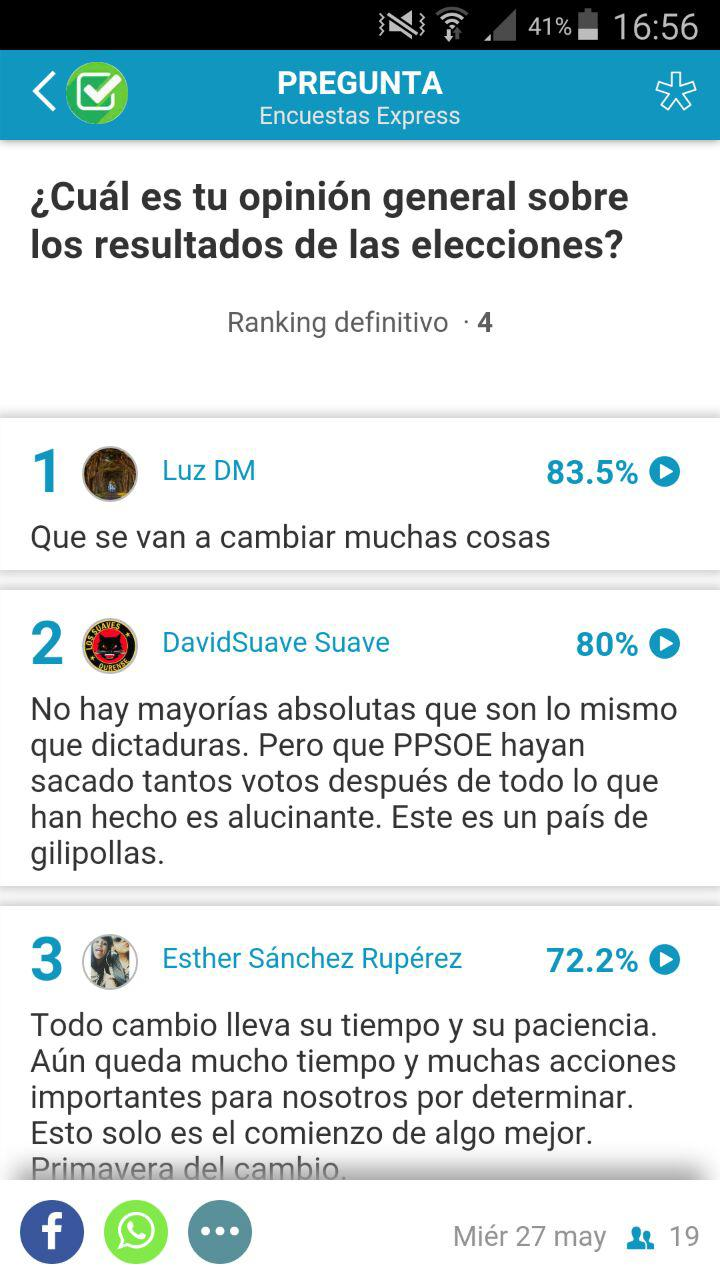
\includegraphics[width=\textwidth]{Media/Captures/appgreeOpenQuestion.jpg}
                \caption{Pregunta Abierta}
                \label{fig:appgreeOpenQuestion}
        \end{subfigure}
        \caption{Capturas de Appgree}\label{fig:appgreeCaptures}
\end{figure}

 - \underline{Aspectos positivos}:

\begin{itemize}
	\item Interfaz limpia de colores planos (blanco y azul) con pantalla principal de ultimas preguntas destacadas.
	\item Organización por canales temáticos de las preguntas.
	\item Opción de marcar canales como favoritos para poder seguirlos y ser notificados de las últimas preguntas añadidas.
\end{itemize}

 - \underline{Aspectos negativos}:

\begin{itemize}
	\item Las preguntas se organizan por antigüedad (activas y no activas) pero se navega de abajo hacia arriba, cuando uno esperaria hacerlo al revés.
	\item Los tipos de preguntas (abiertas, de respuesta múltiple, de sí o no, encuestas...) aparecen todas mezcladas.
\end{itemize}
